\section{Architecture of BIOS Firmware}\label{section-architecture}
\subsection{Overview}
If you interpret BIOS image as close look then it is nothing but the file system which is made in a byte format to be read by low level programming language which is most efficient method to store the data or content.

The concept of initialization of Platform includes the execution of this BIOS image which is stored on the every \gls{soc}

The components which plays role in Platform Initialization are listed below:
\begin{itemize}
	\item Firmware Volume (\gls{fv}) - consists of one or more firmware file systems
	\item Firmware File System (\gls{ffs}) which consists of one or more firmware files
	\item Firmware File - Encapsulated section or leaf section
	\item Reference Layout of Binary
	\item Pre-EFI Initialization (\gls{pei}) PEIM to PEIM Interfaces (PPIs)
	\item Driver Execution Environment (\gls{dxe}) Protocols
\end{itemize}

\subsection{Design of Firmware Storage}
Design of firmware storage elaborates the way that how files needs to be stored and accessed in nonvolatile storage environment. Implementation of any firmware has to support and follow the standard structure for \gls{pi} Firmware Volume and the structure of \gls{ffs}.

\paragraph{Firmware Device} - a persistent physical repository consisting data and/or firmware code. Typically it is a component of flash but may also be any other type of persistent storage. Singular physical firmware device can be partitioned in to multiple other smaller pieces to form many other logical firmware devices from it and vice-versa.


\paragraph{Flash} devices are most usual nonvolatile storage mechanism for firmware volumes. Often, flash devices are partitioned into many sectors or blocks of potentially differing sizes, each along with various runtime characteristics.

In the design of Firmware File System (\gls{ffs}), several observed unique qualities of flash devices are listed below:
\begin{itemize}
	\item Erase operation processed on the basis of sector-by-sector. After ensuring, every bits of sector return their \verb|erase value|\footnote{either all $0$ or all $1$}.
	\item Write operation can be performed on a bit-by-bit basis. i.e. In case erase value is $ 0 $ then bit value $ 0 $ can be changed to $ 1 $.
	\item Only by performing erase operation on the whole flash sector, \verb|non-erase value| can change to \verb|erase value|.
	\item Capable of enable/disable reads and writes to individual flash sectors or the entire flash.
	\item Operations like writes and erases are much longer than reads operation.
	\item Many times places restraints on the trading operations that can be executed while a write or erase is in progress.
\end{itemize}

\subsection{Firmware Volume (\gls{fv})}
The BIOS image is consisting of one or more logical firmware devices known as a Firmware Volume (\gls{fv}). Firmware Volume is the very basic and efficient logical storage mechanism for data and/or code. If you consider file system as a basic unit then firmware volume is unionized into these one or more file system units.
Table \ref{table:firmware-volume-attributes} describes attributes in each firmware volume.

\begin{table}[!htbp]
	\centering
	\renewcommand{\arraystretch}{2}
	\caption{Firmware Volume Attributes}\label{table:firmware-volume-attributes}
	\begin{tabular}{p{4cm} | p{11cm}}
		\textbf{Attribute} & \textbf{Description}
		\\ \hline \hline
		Name & each volume has a unique identifier name having UEFI Globally Unique Identifier (GUID). 
		\\ \hline
		Size & describes total size of all data (includes all information like headers, files and free/reserved space)
		\\ \hline
		Format & describes type of Firmware File System (FFS) which is unionized in construction of the volume.
		\\ \hline
		Memory is Mapped or not? & some volumes may requires to be memory-mapped which determines whether the entire content of the volume can appear at once in the processor's memory address space. 
		\\ \hline
		Sticky Write? & Specifies whether or not special erase cycles requires in order to change value of bits into an erase value from non-erase value
		\\ \hline
		Erase Polarity & In case a volume supports \textit{Sticky Write}, then after processing an erase cycle every bits in the volume will return to this value ($ 0 $ or $ 1 $)
		\\ \hline
		Alignment & A volume is required to be aligned on some power-of-two ($ 2^x $) boundary such that $ minimum >= \text{highest file alignment value} $.
		\\ \hline
		Enable/Disable Read capable status & Decides whether to keep volumes as hidden from readable or not
		\\ \hline
		Enable/Disable Write capable Status & Decides whether to keep volumes as hidden from writable or not
		\\ \hline
		Lock Capable/Status & Volumes could also have their locking mechanism
		\\ \hline
		Read-Lock Capable/Status & Volumes could also have the power to lock their read status
		\\ \hline
		Write-Lock Capable/Status & Volumes could also have the power to lock their write status
		\\ \hline
	\end{tabular}
\end{table}

Apart from this Firmware volumes also consisting of few more information about the correspondence between OEM file types and a \verb|GUID|.

\subsection{Firmware File System (\gls{ffs})}
The logical data payload within firmware volume is known as a Firmware File System (\gls{ffs}) which illustrates the structure of files and free space (if any). To affiliate a driver to firmware volume every firmware file systems contains a globally unique ID (GUID).


\begin{table}[h]
	\centering
	\renewcommand{\arraystretch}{2}
	\caption{Firmware Files Attributes}\label{table:firmware-files-attributes}
	\begin{tabular}{p{4cm} | p{11cm}}
		\textbf{Attribute} & \textbf{Description}
		\\ \hline \hline
		Name & each volume has a unique identifier name having UEFI Globally Unique Identifier (\gls{guid}). Name of the File(s) has to be unique within a same firmware volume.
		\\ \hline
		Type & Type of the individual file which can be Normal, OEM, Debug, FV Specific. More file types information are described in Figure \ref{fig:firmware-file-types}.
		\\ \hline
		Alignment & Every data of file to be aligned on some power-of-two ($ 2^x $) boundary such that these boundaries are founded depending on the alignment of firmware volume.
		\\ \hline
		Size & Describes size of each file which consists of data of size zero or more bytes
		\\ \hline
	\end{tabular}
\end{table}

Firmware files consists of code or raw data or both. Attributes of files are described in Table \ref{table:firmware-files-attributes}.

Integrity check and staged file creation are some extra attribute formats which might spotted in some firmware volume. Firmware File Sections are unit which unionized in a standard fashion to form certain file types for the file data.

OEM file types (described in detail in Figure \ref{fig:firmware-file-types}) enables to support non-standard file types.

PEI phase is responsible to serve the file related services which are carried out using PEI Service Table. On the Other hand the \\ \verb|EFI_FIRMWARE_VOLUME2_PROTOCOL| services which are attached to a volume's handle (\verb|ReadFile|, \verb|ReadSection|, \verb|WriteFile| and \verb|GetNextFile|) are responsible to carried out file related services in DXE phase.

\subsubsection{Firmware File Types}
If you consider an application with file name such as \texttt{XYZ.exe}, in which content format of \verb|XYZ.exe| is implied by the ".exe" in the file name. Based on the situation of operation, this extension normally signals the contents of \verb|XYZ.exe|. The PI Firmware File System characterizes the contents of a file that is returned by the firmware volume interface.

Firmware File System of the Platform Initialization dictates an enumeration of many file types. For example, the type
\verb|EFI_FV_FILETYPE_RAW| implies that the file is a RAW Binary Data. In the same way, files with the type \verb|EFI_FV_FILETYPE_SMM_CORE| supports MM traditional mode .

\begin{figure}[!htbp]
	\centering
	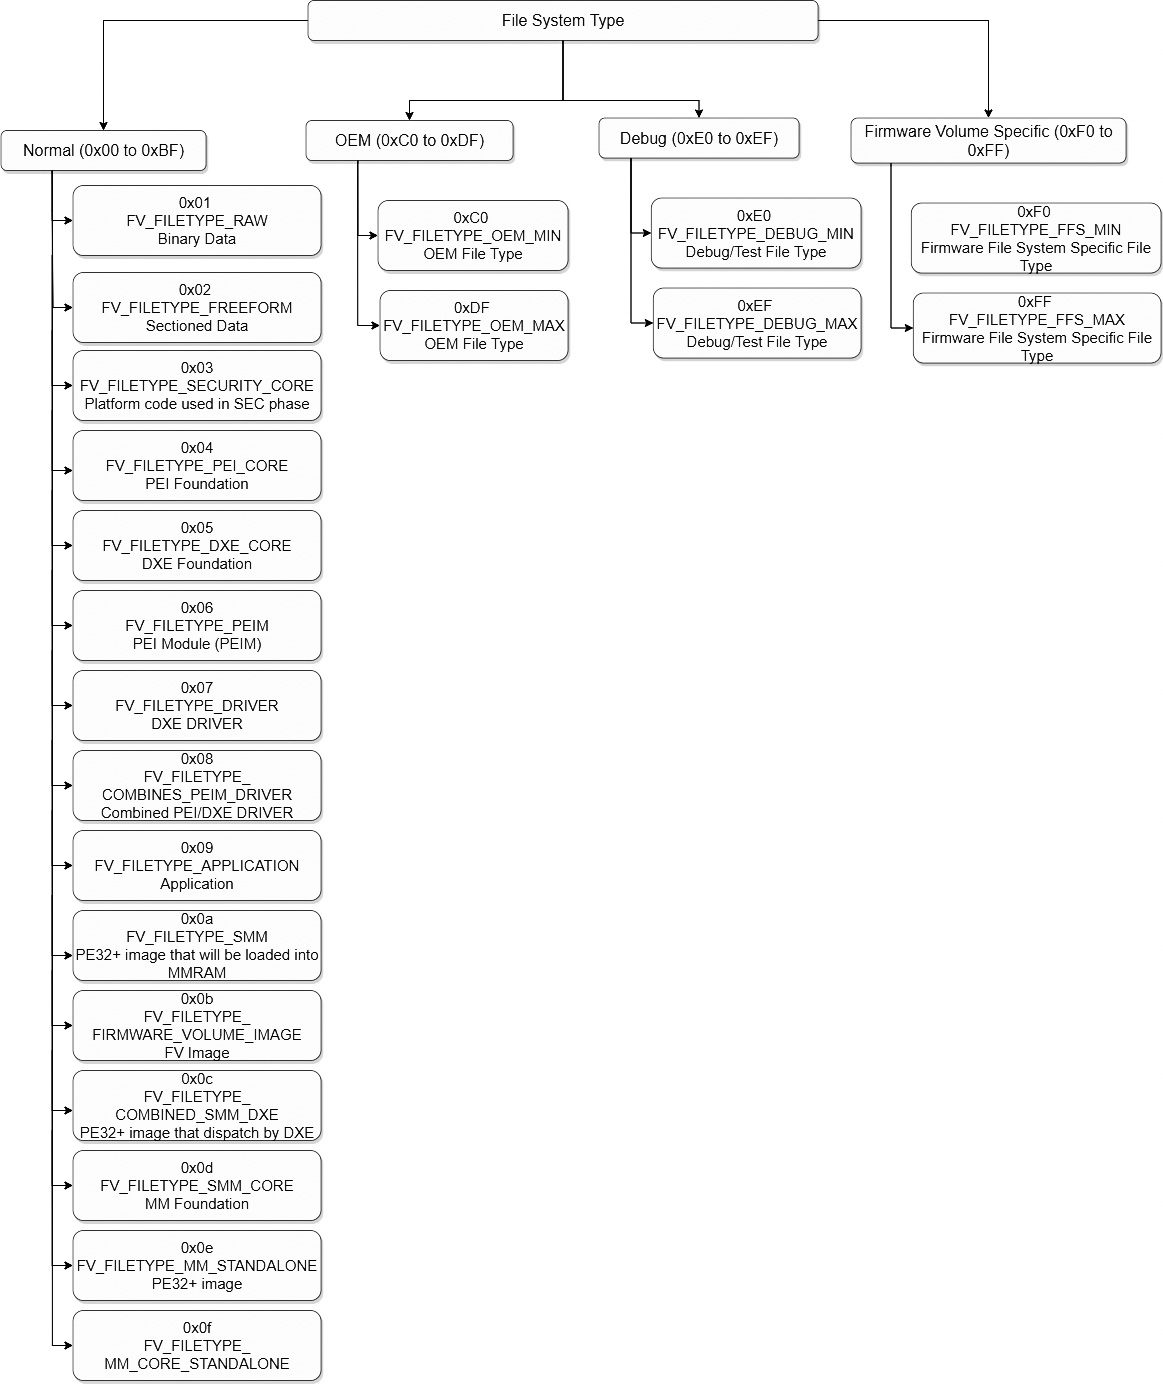
\includegraphics[width=0.9\linewidth]{architecture/firmware-file-type}
	\caption{Firmware File Type}\label{fig:firmware-file-types}
\end{figure}

\subsection{Firmware File Section}
Firmware File Section is individual distinct unit of certain file types which has following attributes:
\begin{table}[!htbp]
	\begin{tabular}{l | p{9cm}}
		Attribute & Description
		\\ \hline \hline
		Type & Each section has type 
		\\ \hline
		Size & describes size of the section
		\\ \hline
	\end{tabular}
\end{table}

However as many as types of sections are present, they eventually fall in one of the below broadly described categories:
\begin{itemize}
	\item \textbf{Encapsulation section} - logical storage consisting of the one or more section.
	The child section(s) which are lying within the encapsulation section (parent section) can be another encapsulation section or a leaf section which are also called relative peers to each other. An encapsulation section never consists of data in itself; however it is just a container that ultimately ends in leaf section(s). Files which are stacked with section can be imagined as tree consisting of nodes (encapsulation section) and	leaves (leaf section). The root which can be interpreted as the file image itself may have a discrete number of sections. Sections that exist in the root have no parent section but are still considered peers.
	
	\item \textbf{Leaf Sections} - Contrary to the encapsulation section, leaf section does contain data and only data within it. Type of section defines which kind of data is stored within the leaf section.
\end{itemize}

\begin{figure}[!htbp]
	\centering
	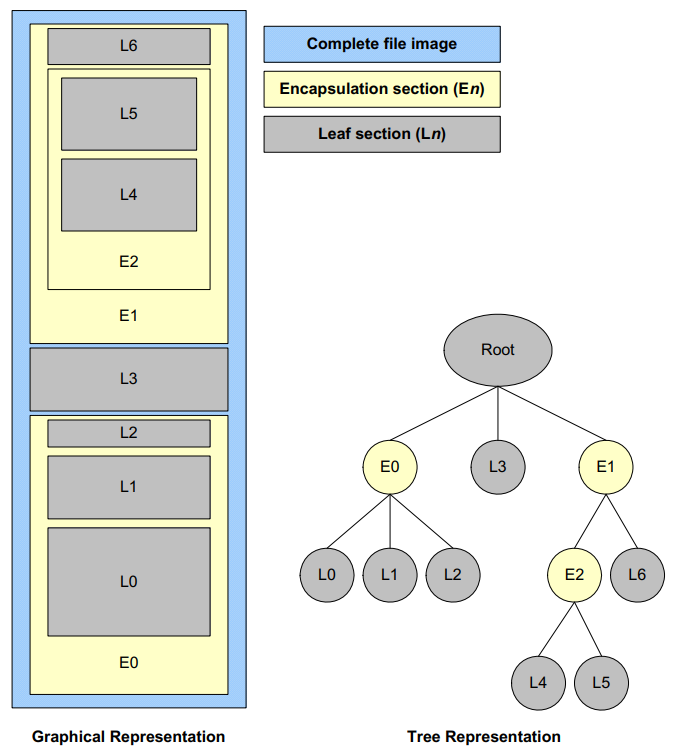
\includegraphics[width=0.9\linewidth]{architecture/firmware-file-system-representation}
	\caption{Example File System Image}\label{fig:architecture-firmware-file-system-representation}
\end{figure}

As illustrated in Figure \ref{fig:architecture-firmware-file-system-representation}, the root which we interpret as the file image has two encapsulation sections which are $ E0 $, $ E1 $ and one leaf section which is $ L3 $. $ E0 $ which is the first encapsulation section possessing three child node which are all leaves ($ L0 $, $ L1 $, and $ L2 $). $ E1 $ is the another encapsulation section which possesses only two children, where one of them is encapsulation ($ E2 $) and the another is the leaf ($ L6 $). $ E2 $ which is the very last encapsulation section consists two children which are both leaves only ($ L4 $ and $ L5 $).

With the help of \verb|FfsFindSectionData|, services related to section are populated with the help of PEI Service Table in the PEI phase. On the other hand \verb|ReadSection| which is attached to service protocol \verb|EFI_FIRMWARE_VOLUME2_PROTOCOL| responsible to populate services related to section during the DXE phase.

\subsection{Firmware File Section Types}
Subjective types of section are described in Table \ref{table:architectural-section-types}.

\begin{table}[!htbp]
	\centering
	\renewcommand{\arraystretch}{1.2}
	\caption{Types of Section}\label{table:architectural-section-types}
	\begin{tabular}{p{7cm} | l | p{5cm}}
		Name of Section & Value & Details
		\\ \hline \hline
		\verb|EFI_SECTION_COMPRESSION| & $ 0x1 $ & non-leaf section containing compressed section(s) within
		\\ \hline
		\verb|EFI_SECTION_GUID_DEFINED| & $ 0x2 $ & non-leaf section which only to be used while in process of build and not for execution
		\\ \hline
		\verb|EFI_SECTION_DISPOSABLE| & $ 0x3 $ & non-leaf section which only to be used while in process of build and not for execution
		\\ \hline
		\verb|EFI_SECTION_PE32| & $ 0x10 $ & Image executable of PE32+
		\\ \hline
		\verb|EFI_SECTION_PIC| & $ 0x11 $ & Code independent of position
		\\ \hline
		\verb|EFI_SECTION_TE| & $ 0x12 $ & Image of Terse Executable
		\\ \hline
		\verb|EFI_SECTION_DXE_DEPEX| & $ 0x13 $ & Expression for DXE driver dependency
		\\ \hline
		\verb|EFI_SECTION_VERSION| & $ 0x14 $ & version of the section - text/numeric
		\\ \hline
		\verb|EFI_SECTION_USER_INTERFACE| & $ 0x15 $ & Human readable and easily interpretable name for driver
		\\ \hline
		\verb|EFI_SECTION_COMPATIBILITY16| & $ 0x16 $ & 16-bit exe of DOS fashion
		\\ \hline
		\verb|EFI_SECTION_FIRMWARE_VOLUME_IMAGE| & $ 0x17 $ & PI Firmware Volume Image
		\\ \hline
		\verb|EFI_SECTION_FREEFORM_SUBTYPE_GUID| & $ 0x18 $ & Raw data with GUID in header to define format
		\\ \hline
		\verb|EFI_SECTION_RAW| & $ 0x19 $ & Raw data
		\\ \hline
		\verb|EFI_SECTION_PEI_DEPEX| & $ 0x1b $ & Expression for PEI driver dependency
		\\ \hline
		\verb|EFI_SECTION_SMM_DEPEX| & $ 0x1c $ & Leaf section which determine the order of dispatch for the MM Traditional driver in SMM.
		\\ \hline
	\end{tabular}
\end{table}

\subsection{PI Architecture Firmware File System Format}
Basic encoding of binary used for PI firmware file, firmware volume and file system is illustrated in this section. Development which carries out the non-vendor firmware files or firmware volumes to be enclosed into the system must have the standard formats. These sections also describes the way features of the standard format mapped into the standard interfaces of DXE and PEI.

The standard format of firmware file and volume also brings in extra dimensions and potential that are used to assure the unity of firmware volume. The standard format is unionized by three different levels: firmware volume, firmware file system, and firmware file.

\begin{figure}[!htbp]
	\centering
	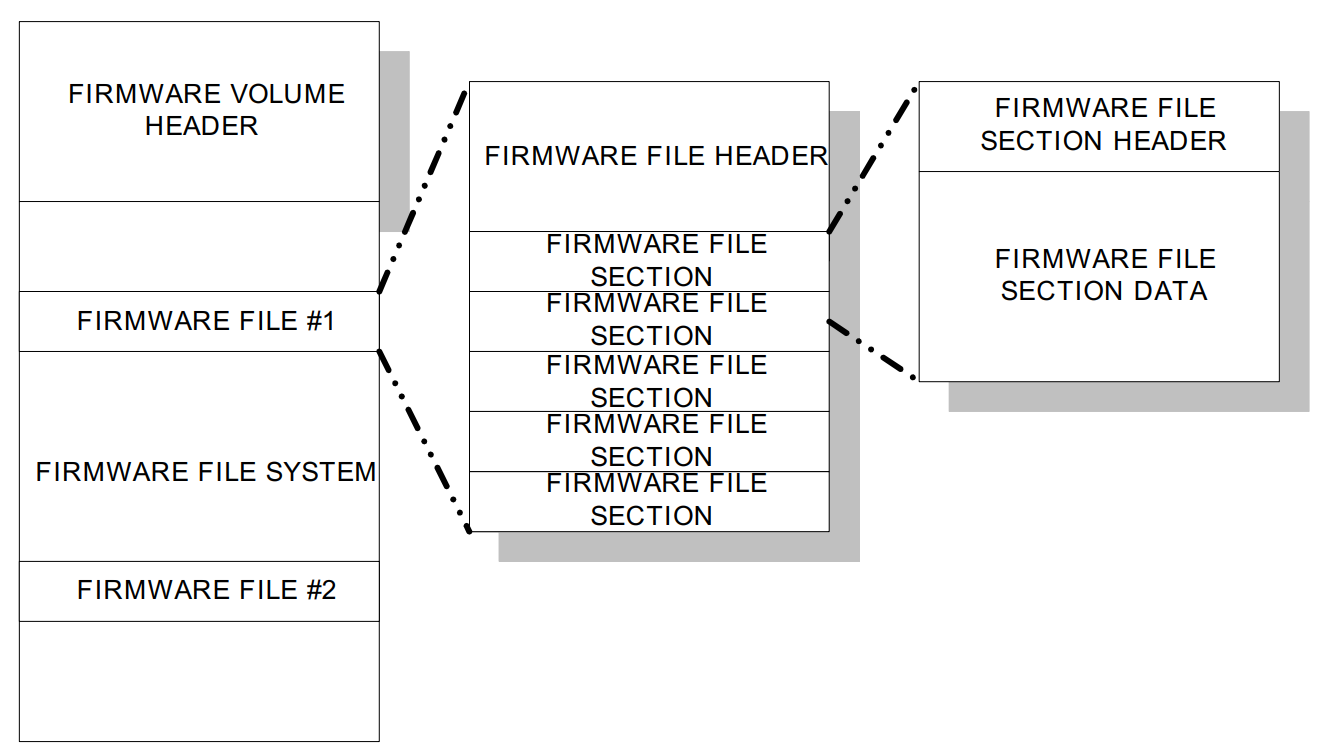
\includegraphics[width=0.8\linewidth]{architecture/the-firmware-volume-format}
	\caption{The Firmware Volume Format}\label{fig:architecture-the-firmware-volume-format}
\end{figure}

The guided formatting of firmware volume (Figure \ref{fig:architecture-the-firmware-volume-format}) made of two parts: 
The FV header and FV data. Header of FV describes every attributes mentioned in “Firmware Volumes” in Table \ref{table:firmware-volume-attributes}. This header also has \gls{guid} which identifies format of the firmware file system utilized to orchestrate data in the firmware volume. The \say{firmware volume header} is compatible with every other firmware file systems except the PI Firmware File System.

\say{Firmware File System format} explains the way the firmware files and free space are conceived inside the firmware volume. However on the other hand \say{Firmware File format} describes how files are organized. The firmware file format made of two parts: the firmware file header and the firmware file data.

\subsubsection{Firmware Volume Format}
The PI Architecture Firmware Volume format key outs the binary structure of a firmware volume. The firmware volume format possesses a FV header followed by the FV data. The FV header is represented by variable \verb|EFI_FIRMWARE_VOLUME_HEADER|.
The format layout of the FV data is described by a GUID. Valid files system GUID values are \verb|EFI_FIRMWARE_FILE_SYSTEM2_GUID| and \verb|EFI_FIRMWARE_FILE_SYSTEM3_GUID|.

\subsubsection{Firmware File System Format}
The PI Architecture Firmware File System is a binary design of logical file storage within firmware volumes. It is a flat file system in which there is no rendering of any directory hierarchy structure. Each and every files lies directly in the root of the storage. Files are stored end to end without any directory entry to explain which files are present. Parsing the information stored in a firmware volume to find a itemization of files exists needs the complete walk through over the firmware volume in and out.

\paragraph{Firmware File System GUID} The firmware volume header has a unique data field for the file system GUID. The two valid FFS file systems are defined by the GUID values in variable \verb|EFI_FIRMWARE_FILE_SYSTEM2_GUID| and \verb|EFI_FIRMWARE_FILE_SYSTEM3_GUID|. In case of the FFS file system, if it does allows files larger than $ 16 \ MB $ along with backward compatibility \verb|EFI_FIRMWARE_FILE_SYSTEM2_GUID| then \verb|EFI_FIRMWARE_FILE_SYSTEM3_GUID| is used.

\paragraph{Volume Top File} known as VTF is a file that has to be presented such that the very last byte of file is also the very last byte of the firmware volume. Irrespective of type of the file, a VTF have to have GUID for the file name which is declared as variable \verb|EFI_FFS_VOLUME_TOP_FILE_GUID|.
Driver cide if Firmware file system has to be exposed of this GUID and infix an alignment pad file as and when needed to assure that the VTF is situated correctly at the top of the firmware volume. Length and alignment of File requirements needs to be coherent with the top of volume so that a write error does occurs and the unwanted firmware volume modification can be prevented.

\subsection{Firmware File Format (\gls{ffs})}
Every FFS files begins with its header data that is aligned on an $ 8-byte $ (which is power-of-two $ 2^3 $) boundary with respect to the origin of the firmware volume. FFS files consists of the below parts:
\begin{itemize}
	\item Header
	\item Data
\end{itemize}

When a zero-length file is created without any data it still has to have header and will consume minimum $ 24 bytes $ of space.

The data (if any) exists in file then it immediately conjugated after the header. How the data within a file
is formed can be identified by the \say{Type} field in the header which can be either of \verb|EFI_FFS_FILE_HEADER| and \verb|EFI_FFS_FILE_HEADER2|.

Figure \ref{fig:architecture-typical-ffs-file-layout-less-than-16MB} exemplifies the typical layout of a (i.e. \verb|EFI_FFS_FILE_HEADER|) \say{PI Architecture Firmware File} $ (\leq 16 Mb) $.

\begin{figure}[!htbp]
	\centering
	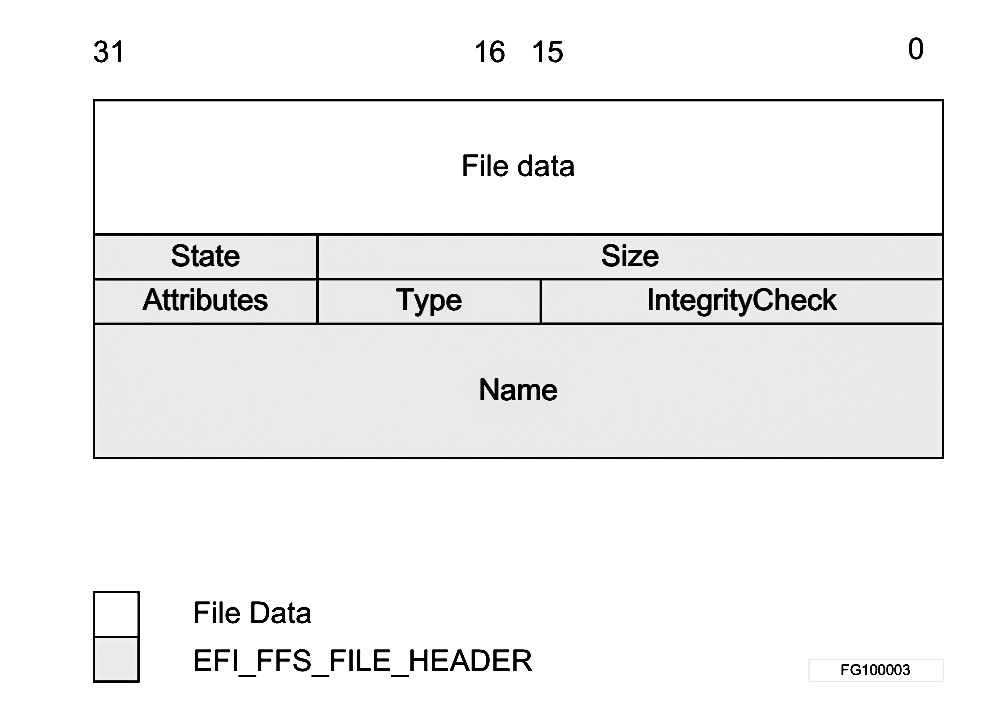
\includegraphics[width=0.8\linewidth]{architecture/typical-ffs-file-layout-less-than-16MB}
	\caption{Layout representation of FFS File Header $ (\leq 16 Mb) $ }\label{fig:architecture-typical-ffs-file-layout-less-than-16MB}
\end{figure}

Figure \ref{fig:architecture-typical-ffs-file-layout-greater-than-16MB} exemplifies the typical layout of \say{PI Architecture Firmware File} $ (> 16 Mb) $.

\begin{figure}[!htbp]
	\centering
	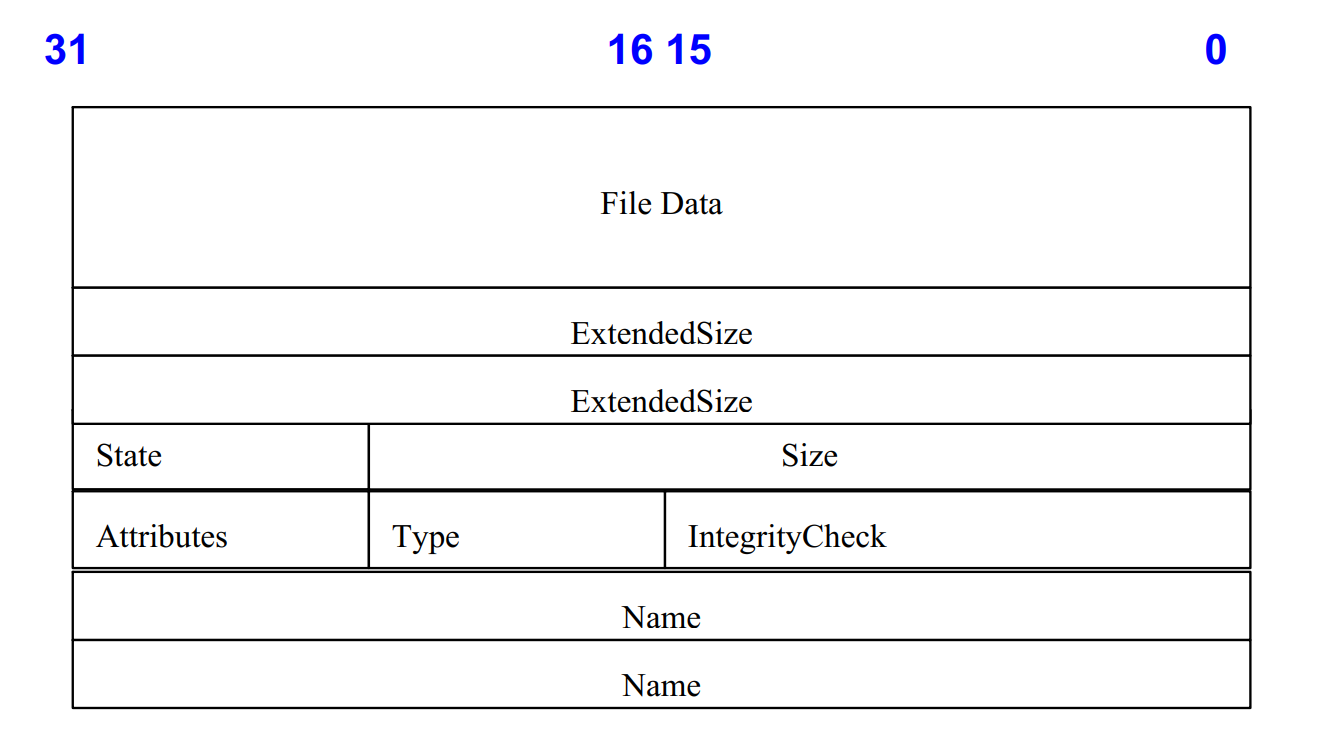
\includegraphics[width=0.8\linewidth]{architecture/typical-ffs-file-layout-greater-than-16MB}
	\caption{Layout representation of FFS File Header 2 layout for files $ (> 16Mb) $}\label{fig:architecture-typical-ffs-file-layout-greater-than-16MB}
\end{figure}


\subsection{Firmware File Section Format}
Storage Data format mechanism of section is described in this section. Each individual section starts with a section header which is followed by the data defined using the section type. Section headers are always aligned at $ 4-byte $ boundaries with respect to the start of the file image. In case of padding required between the section then to achieve the $ 4-byte $
alignment as defined, every bit value of padding is set to zero.
There some section types which are variable in terms of data length and are more precisely represented as data streams instead of data structures.

Irrespective of type of the section, all section headers starts with a $ 24-bit $ integer telling the section size, and $ 8-bit $ section type. The format of the rest of the section header and data is defined by the section type. If size of the section size is $ 0xFFFFFF $ then the size is defined by a $ 32-bit $ integer that follows the $ 32-bit $ section header. Figure \ref{fig:architecture-format-of-a-section-below-16Mb} and Figure \ref{fig:architecture-format-of-a-section-above-16Mb} shows the typical layout of a section data format.

\begin{figure}[!htbp]
	\centering
	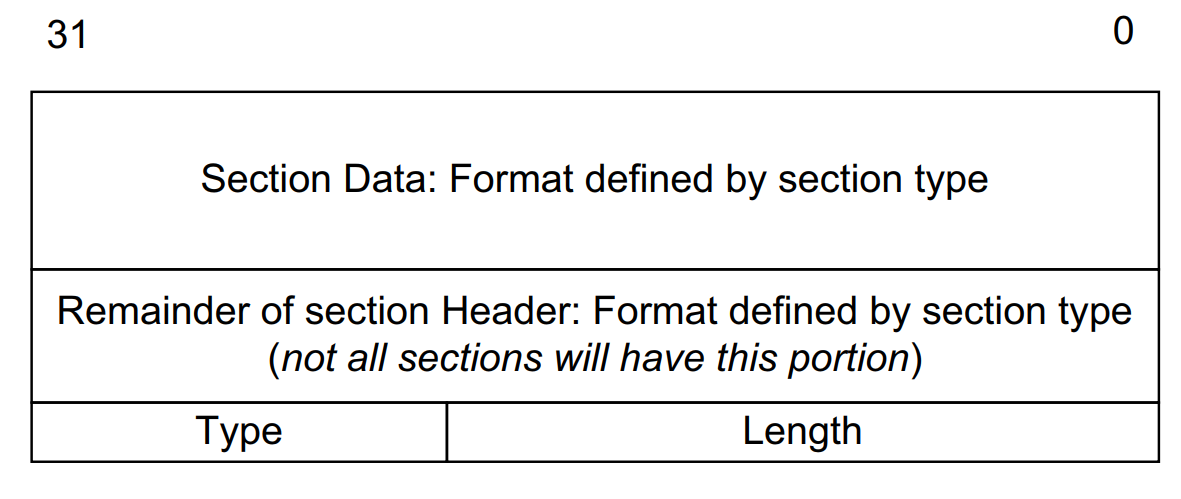
\includegraphics[width=0.8\linewidth]{architecture/format-of-a-section-below-16Mb}
	\caption{Section Header Format when $ size < 16Mb $}\label{fig:architecture-format-of-a-section-below-16Mb}
\end{figure}

\begin{figure}[!htbp]
	\centering
	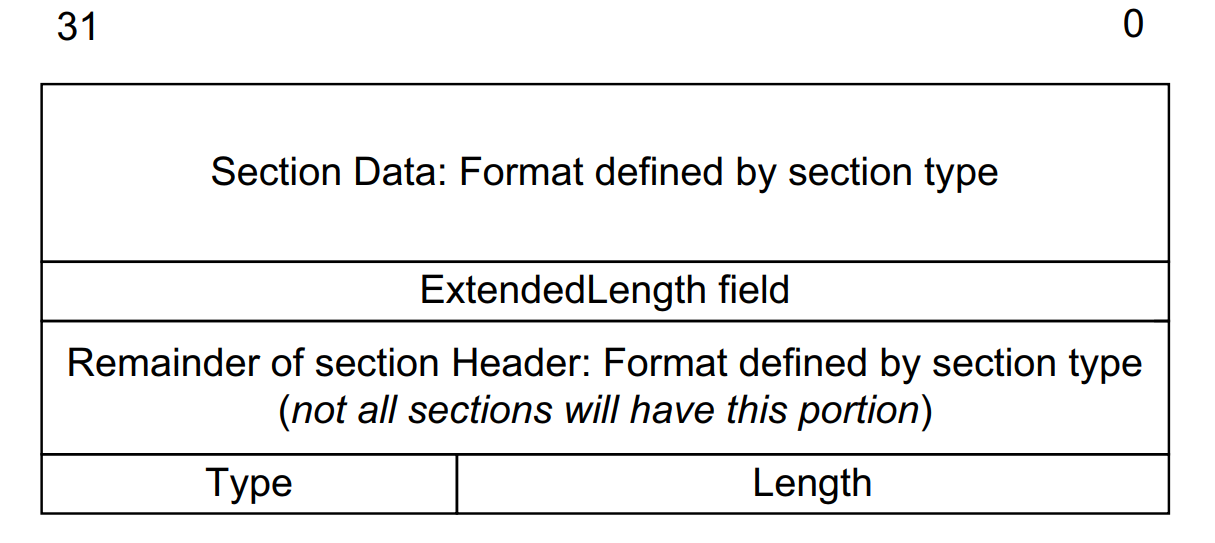
\includegraphics[width=0.8\linewidth]{architecture/format-of-a-section-above-16Mb}
	\caption{Section Header Format of when $ size \geq 16Mb $  using Extended Length field}\label{fig:architecture-format-of-a-section-above-16Mb}
\end{figure}


\subsection{File System Initialization}\label{subsection:file-system-initialization}
To ensure unity of the file system it is mandatory to maintain state byte of each file correctly such that it won't compromised even in case of power failure during operation on any FFS. It is desired that an FFS driver produces an instance of Firmware Volume Protocol so that every normal file operations carried out in that context. Every file operations has to follow all the rules of creation, update, and deletion mentioned in this specification to avoid corruption of the file system.

\subsection{Traversal and Access to Files}
The Security (SEC), PEI, and early DXE code needs to be capable to traverse the FFS such that it's read and execute operation on files carried out before a write-enabled DXE FFS driver is started it's execution so that the FFS may not have any inconsistencies because of any kind of previous system failure. Hence, it has to follow a set of rules to assert the credibility of files before using them. It is not incumbent on SEC, PEI, or the early read-only DXE FFS services to make any effort to perform recovery or modification the file system. If any case exists where execution can not continue because of inconsistencies in file system, a recovery boot must be initiated.

As there is one mutual exclusiveness that the SEC, PEI, and early DXE code can affect without instantiating a recovery boot. This condition can be summoned by any previous system failure such as power failure that come along while a file update on a previous boot. In such case, a failure can cause two files with an identical file name GUID to coexist within the same firmware volume where one of them will have the \verb|EFI_FILE_MARKED_FOR_UPDATE| bit set to its state field but are going to be otherwise totally valid file. The another file may be in unknown state of building up to and including \verb|EFI_FILE_DATA_VALID|. All files used preceding to the initialization of the write-enabled DXE FFS driver must be filtered with this test prior to their use. If this condition is observed, it's tolerable to trigger a recovery boot and allow the recovery DXE to perform the completion of update.

%\inputminted{c}{code/architecture-traversal-and-file-access.c}\label{code:architecture-traversal-and-file-access}


\paragraph{Note} There's no ascertain for redundant files once a file found in the \verb|EFI_FILE_DATA_VALID| state. The condition where two files in same firmware volume coexist having the same file name GUID and both are within the \verb|EFI_FILE_DATA_VALID| state cannot occur if the set of rules for creation and update are strictly followed.

\subsection{File Integrity and State}
File corruption, no matter the cause, must be detectable in order to carried out appropriate steps for file system repair. File corruption can come from various sources but broadly falls into three categories listed below:
\begin{itemize}
	\item Any general failure
	\item Failure on erase
	\item Failure on write
\end{itemize}

A general failure is characterized to be evidently random corruption of the storage media. This corruption can occur because of the design problem or obsolete storage media i.e. This type of failure can be as perceptive as replacing any single bit inside the file content. Using a good design of system along with reliable storage media, general failures can be avoided. However, the FFS enables catching of this kind of failure.

An erase failure happens when a block erase of firmware volume media isn't completed because of any system failure i.e. power failure. As the erase operation is not outlined, it is likely that most of the implementation of FFS that allow file write and delete operations will also develop a mechanism to rectify deleted files and unite free space. In case the operation is not carried out successfully, the file system can be left out in a state which is not consistent. 

Likewise, a write failure takes place when a file system write is in motion and is left incomplete because of any system failure i.e. power failure. This type of failure can lead the file system to be in an inconsistent state.

All of these failures can be traced while FFS initialization is in progress hence depending on the cause of the failure, many recovery schemes can be carried out.



